\chapter{Photometric data}\label{sec:phot}
The photometry database holds \nImages{} reduced exposures (\nImagesOneM{} on the 1-m telescopes) of
\nImageTargets{} targets in \nVisits{} visits (observing blocks), from \firstImage{} to \lastImage{}
(Fig.~\ref{fig:images}). The total open-shutter time is \expImagesH~h. Headers have been read for
\fracImagesHdr\,\% of them.

\begin{figure}[h]
\centering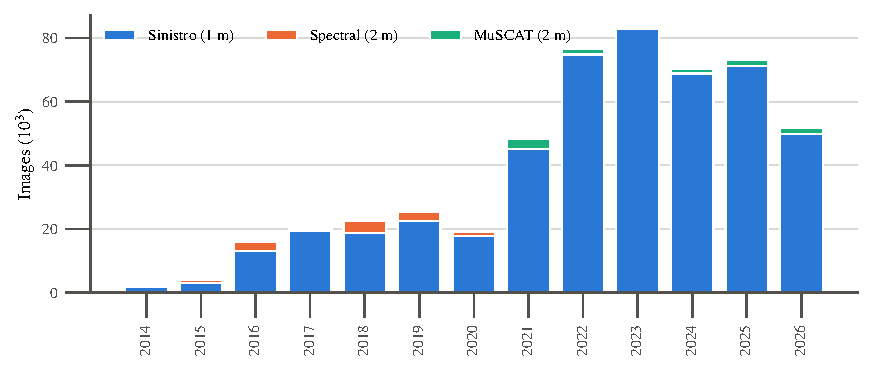
\includegraphics[width=\textwidth]{figures/fig_images_year.pdf}
\caption{Reduced images per year and camera.}\label{fig:images}
\end{figure}

\section{Basic quality of the 1-m images}
The view \texttt{image\_quality} gives, for each exposure, the quantities used for a first quality cut:
filter, object, exposure time, date and MJD, airmass, image size, site, sky brightness, telescope and pixel
scale, plus the BANZAI FWHM. Their distributions for the 1-m images are in Fig.~\ref{fig:quality}: the median
airmass is \medAirmass{} and the median FWHM \medFwhm\,arcsec.

\begin{figure}[h]
\centering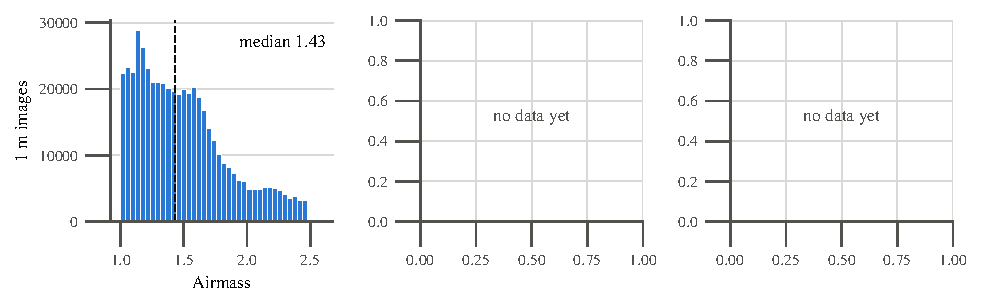
\includegraphics[width=\textwidth]{figures/fig_quality_1m.pdf}
\caption{Airmass, BANZAI image FWHM and header sky brightness of the 1-m images (placeholder sky values of 22.0
excluded). Dashed: median.}\label{fig:quality}
\end{figure}
